\documentclass[a4paper,dvipsnames]{article}

\addtolength{\hoffset}{-2.25cm}
\addtolength{\textwidth}{4.5cm}
\addtolength{\voffset}{-3.25cm}
\addtolength{\textheight}{5cm}
\setlength{\parskip}{0pt}
\setlength{\parindent}{0in}

%----------------------------------------------------------------------------------------
%	PACKAGES AND OTHER DOCUMENT CONFIGURATIONS
%----------------------------------------------------------------------------------------

%----------------------------------------------------------------------------------------
%		Generals
%----------------------------------------------------------------------------------------
\usepackage{fourier}
\usepackage{frcursive}
\usepackage[T1]{fontenc} %Accents handling
\usepackage[utf8]{inputenc} % Use UTF-8 encoding
%\usepackage{microtype} % Slightly tweak font spacing for aesthetics
\usepackage[english, francais]{babel} % Language hyphenation and typographical rules

%----------------------------------------------------------------------------------------
%		Graphics
%----------------------------------------------------------------------------------------
\usepackage{xcolor}
\usepackage{graphicx, multicol} % Enhanced support for graphics
\graphicspath{{FIG/}}
\usepackage{wrapfig}

%----------------------------------------------------------------------------------------
%		Other packages
%----------------------------------------------------------------------------------------
\usepackage{hyperref}
\hypersetup{
	colorlinks=true, %colorise les liens
	breaklinks=true, %permet le retour à la ligne dans les liens trop longs
	urlcolor= bleu3,  %couleur des hyperliens
	linkcolor= bleu3, %couleur des liens internes
	plainpages=false  %pour palier à "Bookmark problems can occur when you have duplicate page numbers, for example, if you have a page i and a page 1."
}
\usepackage{tabularx}
\newcolumntype{M}[1]{>{\arraybackslash}m{#1}} %Defines a scalable column type in tabular
\usepackage{booktabs} % Enhances quality of tables
\usepackage{diagbox} % barre en diagonale dans un tableau
\usepackage{multicol}
\usepackage[explicit]{titlesec}


%----------------------------------------------------------------------------------------
%		Headers and footers
%----------------------------------------------------------------------------------------
\usepackage{fancyhdr} % Headers and footers
\pagestyle{fancy} % All pages have headers and footers
\fancyhead{}\renewcommand{\headrulewidth}{0pt} % Blank out the default header
\renewcommand{\footrulewidth}{0pt}
\fancyfoot[L]{} % Custom footer text
\fancyfoot[C]{\href{https://sacado.xyz/}{sacado.xyz}} % Custom footer text
\fancyfoot[R]{\thepage} % Custom footer text

%----------------------------------------------------------------------------------------
%		Mathematics packages
%----------------------------------------------------------------------------------------
\usepackage{amsthm, amsmath, amssymb} % Mathematical typesetting
\usepackage{marvosym, wasysym} % More symbols
\usepackage[makeroom]{cancel}
\usepackage{xlop}
\usepackage{pgf,tikz,pgfplots}
\pgfplotsset{compat=1.15}
\usetikzlibrary{positioning}
%\usetikzlibrary{arrows}
\usepackage{pst-plot,pst-tree,pst-func, pstricks-add,pst-node,pst-text}
\usepackage{units}
\usepackage{nicefrac}
\usepackage[np]{numprint} %Séparation milliers dans un nombre

%----------------------------------------------------------------------------------------
%		New text commands
%----------------------------------------------------------------------------------------
\usepackage{calc}
\usepackage{boites}
 \renewcommand{\arraystretch}{1.6}

%%%%% Pour les imports.
\usepackage{import}

%%%%% Pour faire des boites
\usepackage[tikz]{bclogo}
\usepackage{bclogo}
\usepackage{framed}
\usepackage[skins]{tcolorbox}
\tcbuselibrary{breakable}
\tcbuselibrary{skins}
\usetikzlibrary{babel,arrows,shadows,decorations.pathmorphing,decorations.markings,patterns}

%%%%% Pour les symboles et les ensembles
\newcommand{\pp}{\leq}
\newcommand{\pg}{\geq}
%\newcommand{\euro}{\eurologo{}}
\newcommand{\R}{\mathbb{R}}
\newcommand{\N}{\mathbb{N}}
\newcommand{\D}{\mathbb{D}}
\newcommand{\Z}{\mathbb{Z}}
\newcommand{\Q}{\mathbb{Q}}
\newcommand{\C}{\mathbb{C}}

%%%%% Pour une double minipage
\newcommand{\mini}[2]{
\begin{minipage}[t]{0.48\linewidth}
#1
\end{minipage}
\hfill
\begin{minipage}[t]{0.48\linewidth}
#2
\end{minipage}
}


%\newcommand\hole[1]{\texttt{\_}}
%\newcommand{\PROP}[1]{\textbf{\underline{#1}}}
%\newcommand{\exercice}{\textcolor{OliveGreen}{Exercice : }}
%\newcommand{\correction}{\textcolor{BurntOrange}{Correction : }}
%\newcommand{\propriete}{\textbf{\underline{Propriété}} : }
%\newcommand{\prop}{\textbf{\underline{Propriété}} : }
%\newcommand{\vocabulaire}{\textbf{\underline{Vocabulaire}} : }
%\newcommand{\voca}{\textbf{\underline{Vocabulaire}} : }

\usepackage{enumitem}
\newlist{todolist}{itemize}{2} %Pour faire des QCM
\setlist[todolist]{label=$\square$} %Pour faire des QCM \begin{todolist} instead of itemize

%----------------------------------------------------------------------------------------
%		Définition de couleur pour geogebra
%----------------------------------------------------------------------------------------
\definecolor{zzttqq}{rgb}{0.6,0.2,0.} %rouge des polygones
\definecolor{qqqqff}{rgb}{0.,0.,1.}
\definecolor{xdxdff}{rgb}{0.49019607843137253,0.49019607843137253,1.}%bleu
\definecolor{qqwuqq}{rgb}{0.,0.39215686274509803,0.} %vert des angles
\definecolor{ffqqqq}{rgb}{1.,0.,0.} %rouge vif
\definecolor{uuuuuu}{rgb}{0.26666666666666666,0.26666666666666666,0.26666666666666666}
\definecolor{qqzzqq}{rgb}{0.,0.6,0.}
\definecolor{cqcqcq}{rgb}{0.7529411764705882,0.7529411764705882,0.7529411764705882} %gris
\definecolor{qqffqq}{rgb}{0.,1.,0.}
\definecolor{ffdxqq}{rgb}{1.,0.8431372549019608,0.}
\definecolor{ffffff}{rgb}{1.,1.,1.}
\definecolor{ududff}{rgb}{0.30196078431372547,0.30196078431372547,1.}

%-------------------------------------------------
%
%	EN TETE
%
%-------------------------------------------------

% Classe
\newcommand{\myClasse}   
{
    6e
}

% Discipline
\newcommand{\myDiscipline}   
{
    Mathématiques
}

% Parcours
\newcommand{\myParcours}
{
  Nombres et Calculs
}

%Titre de la séquence
\newcommand{\myTitle}
{
    \scshape\huge
\textcolor{sacado_purple}{
		Nombres décimaux
}
}

%----------------------------------------------------------------------------------------

%----------------------------------------------------------------------------------------
%		Définition de couleur pour les boites
%----------------------------------------------------------------------------------------
\definecolor{bleu1}{rgb}{0.54,0.79,0.95} %% Bleu
\definecolor{sapgreen}{rgb}{0.4, 0.49, 0}
\definecolor{dvzfxr}{rgb}{0.7,0.4,0.}
\definecolor{beamer}{rgb}{0.5176470588235295,0.49019607843137253,0.32941176470588235} % couleur beamer
\definecolor{preuveRbeamer}{rgb}{0.8,0.4,0}
\definecolor{sectioncolor}{rgb}{0.24,0.21,0.44}
\definecolor{subsectioncolor}{rgb}{0.1,0.21,0.61}
\definecolor{subsubsectioncolor}{rgb}{0.1,0.21,0.61}
\definecolor{info}{rgb}{0.82,0.62,0}
\definecolor{bleu2}{rgb}{0.38,0.56,0.68}
\definecolor{bleu3}{rgb}{0.24,0.34,0.40}
\definecolor{bleu4}{rgb}{0.12,0.20,0.25}
\definecolor{vert}{rgb}{0.21,0.33,0}
\definecolor{vertS}{rgb}{0.05,0.6,0.42}
\definecolor{red}{rgb}{0.78,0,0}
\definecolor{color5}{rgb}{0,0.4,0.58}
\definecolor{eduscol4B}{rgb}{0.19,0.53,0.64}
\definecolor{eduscol4P}{rgb}{0.62,0.12,0.39}

%----------------------------------------------------------------------------------------
%		Définition de couleur pour les boites SACADO
%----------------------------------------------------------------------------------------
\definecolor{sacado_blue}{RGB}{0,129,159} %% Bleu Sacado
\definecolor{sacado_green}{RGB}{59, 157, 38} %% Vert Sacado
\definecolor{sacado_yellow}{RGB}{255,180,0} %% Jaune Sacado
\definecolor{sacado_purple}{RGB}{94,68,145} %% Violet foncé Sacado
\definecolor{sacado_violet}{RGB}{153,117,224} %% Violet clair Sacado
\definecolor{sacado_orange}{RGB}{249,168,100} %% Orange Sacado
\definecolor{ill_frame}{HTML}{F0F0F0}
\definecolor{ill_back}{HTML}{F7F7F7}
\definecolor{ill_title}{HTML}{AAAAAA}


 % Compteurs pour Théorème, Définition, Exemple, Remarque, .....
\newcounter{cpttheo}
\setcounter{cpttheo}{0}
\newcounter{cptdef}
\setcounter{cptdef}{0}
\newcounter{cptmth}
\setcounter{cptmth}{0}
\newcounter{cpttitre}
\setcounter{cpttitre}{0}
 % Exercices
\newcounter{cptapp}
\setcounter{cptapp}{0}
\newcounter{cptex}
\setcounter{cptex}{0}
\newcounter{cptsr}
\setcounter{cptsr}{0}
\newcounter{cpti}
\setcounter{cpti}{0}
\newcounter{cptcor}
\setcounter{cptcor}{0}




%%%%% Pour réinitialiser numéros des paragraphes après une nouvelle partie
\makeatletter
    \@addtoreset{paragraph}{part}
\makeatother


%%%% Titres et sections

\newlength\chapnumb
\setlength\chapnumb{3cm}


% \titleformat{\part}[block] {
 % \normalfont\sffamily\color{violet}}{}{0pt} {
   % \parbox[t]{\chapnumb}{\fontsize{120}{110}\selectfont\ding{110}}
   % \parbox[b]{\dimexpr\textwidth-\chapnumb\relax}{
       % \raggedleft
       % \hfill{{\color{bleu3}\fontsize{40}{30}\selectfont#1}}\\
       % \rule{0.99\textwidth-\chapnumb\relax}{0.4pt}
 % }
% }

% \titleformat{name=\part,numberless}[block]
% {\normalfont\sffamily\color{bleu3}}{}{0pt}
% {\parbox[b]{\chapnumb}{%
  % \mbox{}}%
 % \parbox[b]{\dimexpr\textwidth-\chapnumb\relax}{%
   % \raggedleft%
   % \hfill{{\color{bleu3}\fontsize{40}{30}\selectfont#1}}\\
   % \rule{0.99\textwidth-\chapnumb\relax}{0.4pt}
 % }
% }



% \titleformat{\chapter}[block] {
 % \normalfont\sffamily\color{violet}}{}{0pt} {
   % \parbox[t]{\chapnumb}{ 
     % \fontsize{120}{110}\selectfont\thechapter}
     % \parbox[b]{\textwidth-\chapnumb}{
       % \raggedleft
       % \hfill{{\color{bleu3}\huge#1}}\\  
  % \ifthenelse{\thechapter<10}{\rule{0.99\textwidth-\chapnumb}{0.4pt}}{\rule{0.9\textwidth - \chapnumb}{0.4pt}}
       % \setcounter{cpttitre}{0}
	% \setcounter{cptapp}{0}
	% \setcounter{cptex}{0}
	% \setcounter{cptsr}{0}
	% \setcounter{cpti}{0}
	% \setcounter{cptcor}{0} 
 % }
% }

% \titleformat{name=\chapter,numberless}[block]
% {\normalfont\sffamily\color{bleu3}}{}{0pt}
% {\parbox[b]{\chapnumb}{%
  % \mbox{}}%
 % \parbox[b]{\textwidth-\chapnumb}{%
   % \raggedleft
   % \hfill{{\color{bleu3}\huge#1}}\\
   % \ifthenelse{\thechapter<10}{\rule{0.99\textwidth-\chapnumb}{0.4pt}}{ \rule{0.9\textwidth - \chapnumb}{0.4pt}}
       % \setcounter{cpttitre}{0}
	% \setcounter{cptapp}{0}
	% \setcounter{cptex}{0}
	% \setcounter{cptsr}{0}
	% \setcounter{cpti}{0}
	% \setcounter{cptcor}{0} 
 % }
% }
%
%       
%
%%%%% Personnalisation des numéros des sections
\renewcommand\thesection{\Roman{section}. }
\renewcommand\thesubsection{\hspace{1cm}\arabic{subsection}. }
\renewcommand\thesubsubsection{\hspace{2cm}\alph{subsubsection}. }

\titleformat{\section}[hang]{\color{sacado_purple}{}\normalfont\filright\huge}{}{0.4em}{\textbf{\thesection  #1}}   
% \titlespacing*{\section}{0.2pt}{0ex plus 0ex minus 0ex}{0.3em}
   
\titleformat{\subsection}[hang]{\color{sacado_purple}{}\normalfont\filright\Large}{}{0.4em}{\thesubsection
 #1}            
\titleformat{\subsubsection}[hang]{\color{sacado_purple}{}\normalfont\filright\large}{}{0.4em}{\thesubsubsection
 #1}
\titleformat{\paragraph}[hang]{\color{black}{}\normalfont\filright\normalsize}{}{0.4em}{#1}



%%%%%%%%%%%%%%%%%%%%% Cycle 4
%\newcommand{\Titre}[2]{\section*{#1 
%\ifthenelse{\equal{#2}{1}}   {\hfill{ \ding{182}  \ding{173} \ding{174} } \addcontentsline{toc}{section}{#1 \ding{182}} }%
%{%
%\ifthenelse{\equal{#2}{2}}{\hfill{ \ding{172}  \ding{183} \ding{174} } \addcontentsline{toc}{section}{#1 {\color{purple}\ding{183}}} }{%           
%\hfill{ \ding{172}  \ding{173} \ding{184} } \addcontentsline{toc}{section}{#1 {\color{orange}\ding{184}}}% 
%}%
%}%
%}
%}


%%%%%%%%%%%%%%%%%%%%% Cycle 4
\newcommand{\Titre}[2]{\section*{#1 
\ifthenelse{\equal{#2}{1}}   {\hfill{ \ding{182}  \ding{173} \ding{174} } \addcontentsline{toc}{section}{#1 \, \ding{182}} }%
{% sinon
\ifthenelse{\equal{#2}{1,5}}   {\hfill{ \ding{182}  \ding{183} \ding{174} } \addcontentsline{toc}{section}{#1 \, \ding{182} {\color{purple}\ding{183}}} }%
{% sinon
\ifthenelse{\equal{#2}{2}}   {\hfill{ \ding{172}  \ding{183} \ding{174} } \addcontentsline{toc}{section}{#1 \, {\color{purple}\ding{183}}} }
{% sinon
\ifthenelse{\equal{#2}{2,5}}   {\hfill{ \ding{172}  \ding{183} \ding{184} } \addcontentsline{toc}{section}{#1 \, {\color{purple}\ding{183}}  {\color{orange}\ding{184}}} }%
{% sinon
\hfill{ \ding{172}  \ding{173} \ding{184} } \addcontentsline{toc}{section}{#1 \,{\color{orange}\ding{184}}}% 
}%
}%
}%
}%
}%
}

%%%%%%%%%%%%% Titre
\newenvironment{titre}[2][]{%
\vspace{0.5cm}
\begin{tcolorbox}[enhanced, lifted shadow={0mm}{0mm}{0mm}{0mm}%
{black!60!white}, attach boxed title to top left={xshift=110mm, yshift*=-3mm}, coltitle=violet, colback=bleu3!25!white, boxed title style={colback=white!100}, colframe=bleu3,title=\stepcounter{cpttitre} \textbf{Fiche \thecpttitre}. #1 #2 ]}
{%
\end{tcolorbox}
\par}



%%%%%%%%%%%%% Définitions
\newenvironment{Def}[1][]{%
\medskip \begin{tcolorbox}[widget,colback=sacado_violet!0,colframe=sacado_violet!75,
adjusted title= \stepcounter{cptdef} Définition \thecptdef . {#1} ]}
{%
\end{tcolorbox}\par}


\newenvironment{DefT}[2][]{%
\medskip \begin{tcolorbox}[widget,colback=sacado_violet!0,colframe=sacado_violet!75,
adjusted title= \stepcounter{cptdef} Définition \thecptdef . {#1} \textit{#2}]}
{%
\end{tcolorbox}\par}

%%%%%%%%%%%%% Proposition
\newenvironment{Prop}[1][]{%
\medskip \begin{tcolorbox}[widget,colback=sacado_blue!0,colframe=sacado_blue!75!black,
adjusted title= \stepcounter{cpttheo} Proposition \thecpttheo . {#1} ]}
{%
\end{tcolorbox}\par}

%%%%%%%%%%%%% Propriétés
\newenvironment{Pp}[1][]{%
\medskip \begin{tcolorbox}[widget,colback=sacado_blue!0,colframe=sacado_blue!75!black,
adjusted title= \stepcounter{cpttheo} Propriété \thecpttheo . {#1}]}
{%
\end{tcolorbox}\par}

\newenvironment{PpT}[2][]{%
\medskip \begin{tcolorbox}[widget,colback=sacado_blue!0,colframe=sacado_blue!75!black,
adjusted title= \stepcounter{cpttheo} Propriété \thecpttheo . {#1} #2]}
{%
\end{tcolorbox}\par}

\newenvironment{Pps}[1][]{%
\medskip \begin{tcolorbox}[widget,colback=sacado_blue!0,colframe=sacado_blue!75!black,
adjusted title= \stepcounter{cpttheo} Propriétés \thecpttheo . {#1}]}
{%
\end{tcolorbox}\par}

%%%%%%%%%%%%% Théorèmes
\newenvironment{ThT}[2][]{% théorème avec titre
\medskip \begin{tcolorbox}[widget,colback=sacado_blue!0,colframe=sacado_blue!75!black,
adjusted title= \stepcounter{cpttheo} Théorème \thecpttheo . {#1} #2]}
{%
\end{tcolorbox}\par}

\newenvironment{Th}[1][]{%
\medskip \begin{tcolorbox}[widget,colback=sacado_blue!0,colframe=sacado_blue!75!black,
adjusted title= \stepcounter{cpttheo} Théorème \thecpttheo . {#1}]}
{%
\end{tcolorbox}\par}

%%%%%%%%%%%%% Règles
\newenvironment{Reg}[1][]{%
\medskip \begin{tcolorbox}[widget,colback=sacado_blue!0,colframe=sacado_blue!75!black,
adjusted title= \stepcounter{cpttheo} Règle \thecpttheo . {#1}]}
{%
\end{tcolorbox}\par}

%%%%%%%%%%%%% REMARQUES
\newenvironment{Rq}[1][]{%
\begin{bclogo}[couleur=sacado_orange!0, arrondi =0.15, noborder=true, couleurBarre=sacado_orange, logo = \bcinfo ]{ 
{\color{info}\normalsize{Remarque#1}}}}
{%
\end{bclogo}
\par}


\newenvironment{Rqs}[1][]{%
\begin{bclogo}[couleur=sacado_orange!0, arrondi =0.15, noborder=true, couleurBarre=sacado_orange, logo = \bcinfo ]{ 
{\color{info}\normalsize{Remarques#1}}}}
{%
\end{bclogo}
\par}

%%%%%%%%%%%%% EXEMPLES
\newenvironment{Ex}[1][]{%
\begin{bclogo}[couleur=sacado_yellow!15, arrondi =0.15, noborder=true, couleurBarre=sacado_yellow, logo = \bclampe ]{ 
\normalsize{Exemple#1}}}
{%
\end{bclogo}
\par}




%%%%%%%%%%%%% Preuve
\newenvironment{Pv}[1][]{%
\begin{tcolorbox}[breakable, enhanced,widget, colback=sacado_blue!10!white,boxrule=0pt,frame hidden,
borderline west={1mm}{0mm}{sacado_blue!75}]
\textbf{Preuve#1 : }}
{%
\end{tcolorbox}
\par}


%%%%%%%%%%%%% PreuveROC
\newenvironment{PvR}[1][]{%
\begin{tcolorbox}[breakable, enhanced,widget, colback=sacado_blue!10!white,boxrule=0pt,frame hidden,
borderline west={1mm}{0mm}{sacado_blue!75}]
\textbf{Preuve (ROC)#1 : }}
{%
\end{tcolorbox}
\par}


%%%%%%%%%%%%% Compétences
\newenvironment{Cps}[1][]{%
\vspace{0.4cm}
\begin{tcolorbox}[enhanced, lifted shadow={0mm}{0mm}{0mm}{0mm}%
{black!60!white}, attach boxed title to top left={xshift=5mm, yshift*=-3mm}, coltitle=white, colback=white, boxed title style={colback=sacado_green!100}, colframe=sacado_green!75!black,title=\textbf{Compétences associées#1}]}
{%
\end{tcolorbox}
\par}

%%%%%%%%%%%%% Compétences Collège
\newenvironment{CpsCol}[1][]{%
\vspace{0.4cm}
\begin{tcolorbox}[breakable, enhanced,widget, colback=white ,boxrule=0pt,frame hidden,
borderline west={2mm}{0mm}{bleu3}]
\textbf{#1}}
{%
\end{tcolorbox}
\par}




%%%%%%%%%%%%% Attendus
\newenvironment{Ats}[1][]{%
\vspace{0.4cm}
\begin{tcolorbox}[enhanced, lifted shadow={0mm}{0mm}{0mm}{0mm}%
{black!60!white}, attach boxed title to top left={xshift=5mm, yshift*=-3mm}, coltitle=white, colback=white, boxed title style={colback=sacado_green!100}, colframe=sacado_green!75!black,title=\textbf{Attendus du chapitre#1}]}
{%
\end{tcolorbox}
\par}

%%%%%%%%%%%%% Méthode
\newenvironment{Mt}[1][]{%
\vspace{0.4cm}
\begin{bclogo}[couleur=sacado_blue!0, arrondi =0.15, noborder=true, couleurBarre=bleu3, logo = \bccrayon ]{ 
\normalsize{{\color{bleu3}Méthode #1}}}}
{%
\end{bclogo}
\par}


%%%%%%%%%%%%% Méthode en vidéo
\newcommand{\MtV}[2]{\vspace{0.4cm} \colorbox{sacado_blue!0}{\hspace{0.2 cm}\tikz\node[rounded corners=1pt,draw] {\color{red}$\blacktriangleright$}; \quad  \href{https://youtu.be/#1?rel=0}{\raisebox{0.8mm}{{\color{red}\textbf{Méthode en vidéo : #2}}}}}}


%%%%%%%%%%%%% A voir (AV) : Lien externe + vidéo non Youtube
\newcommand{\AV}[2]{\vspace{0.4cm} \colorbox{bleu1!0}{\hspace{0.2 cm}\tikz\node[rounded corners=1pt,draw] {\color{red}$\blacktriangleright$}; \quad  \href{#1}{\raisebox{0.8mm}{{\color{red}\textbf{#2}}}}}}


%%%%%%%%%%%%% Etymologie
\newenvironment{Ety}[1][]{%
\begin{bclogo}[couleur=sacado_green!0, arrondi =0.15, noborder=true, couleurBarre=sacado_green, logo = \bcplume ]{ 
\normalsize{{\color{sacado_green}Étymologie#1}}}}
{%
\end{bclogo}
\par}


%%%%%%%%%%%%% Notation
\newenvironment{Nt}[1][]{%
\begin{bclogo}[couleur=sacado_violet!0, arrondi =0.15, noborder=true, couleurBarre=sacado_violet!75, logo = \bccrayon ]{ 
\normalsize{{\color{violet!75}Notation#1}}}}
{%
\end{bclogo}
\par}
%%%%%%%%%%%%% Histoire
%\newenvironment{His}[1][]{%
%\begin{bclogo}[couleur=brown!30, arrondi =0.15, noborder=true, couleurBarre=brown, logo = \bcvaletcoeur ]{ 
%\normalsize{{\color{brown}Histoire des mathématiques#1}}}}
%{%
%\end{bclogo}
%\par}

\newenvironment{His}[1][]{%
\vspace{0.4cm}
\begin{tcolorbox}[enhanced, lifted shadow={0mm}{0mm}{0mm}{0mm}%
{brown!60!white}, attach boxed title to top left={xshift=5mm, yshift*=-3mm}, coltitle=white, colback=white, boxed title style={colback=brown!100}, colframe=brown!75!black,title=\textbf{Histoire des mathématiques#1}]}
{%
\end{tcolorbox}
\par}

%%%%%%%%%%%%% Attention
\newenvironment{Att}[1][]{%
\begin{bclogo}[couleur=red!0, arrondi =0.15, noborder=true, couleurBarre=red, logo = \bcattention ]{ 
\normalsize{{\color{red}Attention. #1}}}}
{%
\end{bclogo}
\par}


%%%%%%%%%%%%% Conséquence
\newenvironment{Cq}[1][]{%
\textbf{Conséquence #1}}
{%
\par}

%%%%%%%%%%%%% Vocabulaire
\newenvironment{Voc}[1][]{%
\setlength{\logowidth}{10pt}
%\begin{footnotesize}
\begin{bclogo}[ noborder , couleur=white, logo =\bcbook]{#1}}
{%
\end{bclogo}
%\end{footnotesize}
\par}


%%%%%%%%%%%%% Video
\newenvironment{Vid}[1][]{%
\setlength{\logowidth}{12pt}
\begin{bclogo}[ noborder , couleur=white,barre=none, logo =\bcoeil]{#1}}
{%
\end{bclogo}
\par}


%%%%%%%%%%%%% Syntaxe
\newenvironment{Syn}[1][]{%
\begin{bclogo}[couleur=violet!0, arrondi =0.15, noborder=true, couleurBarre=violet!75, logo = \bcicosaedre ]{ 
\normalsize{{\color{violet!75}Syntaxe#1}}}}
{%
\end{bclogo}
\par}

%%%%%%%%%%%%% Auto évaluation
\newenvironment{autoeval}[1][]{%
\vspace{0.4cm}
\begin{tcolorbox}[enhanced, lifted shadow={0mm}{0mm}{0mm}{0mm}%
{black!60!white}, attach boxed title to top left={xshift=5mm, yshift*=-3mm}, coltitle=white, colback=white, boxed title style={colback=sacado_green!100}, colframe=sacado_green!75!black,title=\textbf{J'évalue mes compétences#1}]}
{%
\end{tcolorbox}
\par}


\newenvironment{autotest}[1][]{%
\vspace{0.4cm}
\begin{tcolorbox}[enhanced, lifted shadow={0mm}{0mm}{0mm}{0mm}%
{red!60!white}, attach boxed title to top left={xshift=5mm, yshift*=-3mm}, coltitle=white, colback=white, boxed title style={colback=red!100}, colframe=red!75!black,title=\textbf{Pour faire le point #1}]}
{%
\end{tcolorbox}
\par}

\newenvironment{ExOApp}[1][]{% Exercice d'application direct
\vspace{0.4cm}
\begin{tcolorbox}[enhanced, lifted shadow={0mm}{0mm}{0mm}{0mm}%
{red!60!white}, attach boxed title to top left={xshift=5mm, yshift*=-3mm}, coltitle=white, colback=white, boxed title style={colback=sacado_green!100}, colframe=sacado_green!75!black,title=\textbf{Application #1}]}
{%
\end{tcolorbox}
\par}

\newenvironment{ExOInt}[1][]{% Exercice d'application direct
\vspace{0.4cm}
\begin{tcolorbox}[enhanced, lifted shadow={0mm}{0mm}{0mm}{0mm}%
{red!60!white}, attach boxed title to top left={xshift=5mm, yshift*=-3mm}, coltitle=white, colback=white, boxed title style={colback=sacado_green!50}, colframe=sacado_green!75!black,title=\textbf{Exercice #1}]}
{%
\end{tcolorbox}
\par}

%Illustrations
\newtcolorbox{Illqr}[1]{
  enhanced,
  colback=white,
  colframe=ill_frame,
  colbacktitle=ill_back,
  coltitle=ill_title,
  title=\textbf{Illustration},
  boxrule=1pt, % épaisseur du trait à 1pt
  center,
  overlay={
    \node[anchor=south east, inner sep=0pt,xshift=-1pt,yshift=2pt,fill=white] at (frame.south east) {\fancyqr[height=1cm]{#1}};
  },
  after=\par,
  before=\vspace{0.4cm},
}

\newtcolorbox{Ill}{
  enhanced,
  colback=white,
  colframe=ill_frame,
  colbacktitle=ill_back,
  coltitle=ill_title,
  title=\textbf{Illustration},
  boxrule=1pt, % épaisseur du trait à 1pt
  center,
  after=\par,
  before=\vspace{0.4cm},
}

%%%%%%%%%%%%%% Propriétés
%\newenvironment{Pp}[1][]{%
%\medskip \begin{tcolorbox}[widget,colback=sacado_blue!0,colframe=sacado_blue!75!black,
%adjusted title= \stepcounter{cpttheo} Propriété \thecpttheo . {#1}]}
%{%
%\end{tcolorbox}\par}

%%%%% Pour réinitialiser numéros des chapitres après une nouvelle partie
% \makeatletter
    % \@addtoreset{section}{part}
% \makeatother

% \newcommand{\EPC}[3]{ % Exercice par compétence de niveau 1
% \ifthenelse{\equal{#1}{1}}
% {%condition2 vraie
% \vspace{0.4cm}
% \stepcounter{cptex}
% \tikz\node[rounded corners=0pt,draw,fill=bleu2]{\color{white}\textbf{ \thecptex}}; \quad  {\color{bleu2}\textbf{#3}}
% \input{#2}
% }% fin condition2 vraie
% {%condition2 fausse
% \vspace{0.4cm}
% \stepcounter{cptex}
% \tikz\node[rounded corners=2pt,draw,fill=eduscol4P]{\color{white}\textbf{ \thecptex}}; \quad  {\color{eduscol4P} \textbf{En temps libre.} \textbf{ #3}} 
% \input{#2}
% }% fin condition2 fausse
% } % fin de la procédure

\begin{document}

%-------------------------------
%	TITLE SECTION
%-------------------------------

\fancyhead[C]{}
\hrule \medskip % Upper rule
\begin{minipage}{0.295\textwidth} 
\raggedright
%\footnotesize
Classe \myClasse \hfill\\
\myDiscipline \hfill\\
\myParcours \hfill\\
\end{minipage}
\begin{minipage}{0.4\textwidth} 
\centering 
\large 
\myTitle \\ 
%\normalsize 
%\mySubTitle \\ 
\end{minipage}
\begin{minipage}{0.295\textwidth} 
\raggedleft
\href{https://sacado.xyz/}{
\includegraphics[width=.2\linewidth]{sacadoA1.png}}
%\myAnnee \hfill\\
\end{minipage}
\medskip\hrule 

%-------------------------------
%	CONTENTS
%-------------------------------

\section{Mesurer et comparer des longueurs.}

\section{Le système métrique.}

\begin{His}
%\begin{wrapfigure}{l}{0.3\linewidth}
%\centering
%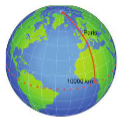
\includegraphics[width=\linewidth]{terre.PNG}
%\end{wrapfigure}
En $1790$, l'Assemblée nationale française décide d'établir un système de mesure unique. Il faut une mesure "pour tous les temps et pour tous les peuples". De nombreu.x.ses savant.e.s sont associé.e.s à ce projet. La Terre est alors choisie comme référence et le mètre défini comme la \textit{dix-millionième} partie du quart du méridien terrestre. \textbf{Pierre Méchain} ($1744-1804$) et \textbf{Jean-Baptiste Delambre} ($1749-1822$), astronomes et mathématiciens, déterminent une mesure précise de la longuer du méridien en $1798$. En $1799$, le mètre étalon est considéré comme définitif, il est déposé aux Archives nationales.
\end{His}

\begin{Def}
Le \textbf{système métrique} est un \textbf{système décimal} :\\
\[1\, m=10\, dm \hspace{1cm} 1\, dm=10\, cm \hspace{1cm}1\, cm=10\, mm\]
\end{Def}

\begin{Mt}
On peut se servir d'un tableau de conversion.
\begin{center}
\begin{tabular}{c|c|c|c|c|c|c}
    \textcolor{red}{kilo}mètre & \textcolor{red}{hecto}mètre & \textcolor{red}{déca}mètre & mètre & \textcolor{red}{déci}mètre & \textcolor{red}{centi}mètre & \textcolor{red}{milli}mètre  \\ \hline 
    \textcolor{red}{k}m & \textcolor{red}{h}m & \textcolor{red}{da}m & m & \textcolor{red}{d}m & \textcolor{red}{c}m & \textcolor{red}{m}m \\ \hline
    \(1 km = 1 000 m\) & \(1 hm = 100 m\) & \(1 dam = 10 m\) & \(1 m\) & \(1 dm = 0,1 m\) & \(1 cm = 0,01 m\) & \(1 mm = 0,001 m\)
\end{tabular}
\end{center}
\end{Mt}

\begin{ExOApp}[]
Convertir les longueurs suivantes
\[1 \,cm = ... \,m \hspace{1cm} 45 \,km = ... \,cm \hspace{1cm} 100 \,mm = ... \,dam \hspace{1cm} 20 \,cm = ... \,dm \hspace{1cm} 4456 \,m = ... \,m\] \[12 \,hm = ... \,mm \hspace{1cm} 0,0033 \,km = ... \,mm \hspace{1cm} 0,005 \,mm = ... \,m \hspace{1cm} 1145 \,cm = ... \,m \hspace{1cm} 45,78 \,m = ... \,dm\]
\end{ExOApp}

\section{Périmètre d'une figure.}

\begin{Def}
Le périmètre d'une figure est la longueur de son contour.
\end{Def}

\begin{Rq}
Le périmètre est une longueur, il s'exprime donc à l'aide d'une unité de longueur.
\end{Rq}

\section{Mesurer, calculer le périmètre d'un polygone.}

\begin{Mt}
Pour calculer le périmètre d'un polygone il suffit d'ajouter les longueurs de ses côtés exprimées dans la même unité.
\end{Mt}

\begin{ExOApp}
\begin{enumerate}

\item Reporter sur une demi-droite le périmètre de la figure à l'aide d'un compas ci-dessous puis le mesurer.
\begin{center}
\begin{tikzpicture}[line cap=round,line join=round,x=0.7cm,y=0.7cm]
\clip(5.58,-2.36) rectangle (12.32,3.28);
\draw [line width=1.pt,color=zzttqq] (5.9,1.04)-- (10.42,3.02);
\draw [line width=1.pt,color=zzttqq] (10.42,3.02)-- (11.94,-1.94);
\draw [line width=1.pt,color=zzttqq] (11.94,-1.94)-- (7.74,-1.14);
\draw [line width=1.pt,color=zzttqq] (7.74,-1.14)-- (5.9,1.04);
%\begin{scriptsize}
\draw [fill=ududff] (5.9,1.04) circle (2.pt);
\draw [fill=ududff] (10.42,3.02) circle (2.pt);
%\draw[color=black] (8.52,1.91) node {$4.9$};
\draw [fill=ududff] (11.94,-1.94) circle (2.pt);
%\draw[color=black] (11.58,0.85) node {$5.2$};
\draw [fill=ududff] (7.74,-1.14) circle (2.pt);
%\draw[color=black] (9.8,-1.11) node {$4.3$};
%\draw[color=black] (7.34,0.05) node {$2.9$};
%\end{scriptsize}
\end{tikzpicture}
\end{center}
\item Calculer le périmètre de la figure ci-dessous :\\
\begin{center}
\begin{tikzpicture}[line cap=round,line join=round,x=1.0cm,y=1.0cm]
\clip(-0.2806258071319262,-0.5469861082594564) rectangle (4.446308277251622,3.057396586133171);
\draw [line width=1.pt,color=zzttqq] (0.,0.01527280802708741)-- (0.,2.5);
\draw [line width=1.pt,color=zzttqq] (-0.045818424081262174,1.2285453939796842) -- (0.04581842408126196,1.2285453939796842);
\draw [line width=1.pt,color=zzttqq] (-0.045818424081262174,1.2867274140474028) -- (0.04581842408126196,1.2867274140474028);
\draw [line width=1.pt,color=zzttqq] (0.,2.5)-- (2.5,2.5);
\draw [line width=1.pt,color=zzttqq] (1.2209089899661407,2.5458184240812622) -- (1.2209089899661407,2.4541815759187378);
\draw [line width=1.pt] (1.279091010033859,2.5458184240812622) -- (1.279091010033859,2.4541815759187378);
\draw [line width=1.pt,color=zzttqq] (2.5,2.5)-- (2.5,1.5);
\draw [line width=1.pt,color=zzttqq] (2.5,1.5)-- (4.,1.5);
\draw [line width=1.pt,color=zzttqq] (3.25,1.545818424081262) -- (3.25,1.4541815759187375);
\draw [line width=1.pt,color=zzttqq] (4.,1.5)-- (4.,0.);
\draw [line width=1.pt,color=zzttqq] (4.045818424081262,0.75) -- (3.9541815759187378,0.75);
\draw [line width=1.pt,color=zzttqq] (4.,0.)-- (0.,0.01527280802708741);
%\begin{scriptsize}
\draw [fill=ududff] (0.,0.01527280802708741) circle (2pt);
\draw[color=ududff] (-0.028624474684984226,-0.3384384935348683) node {$A$};
\draw [fill=ududff] (0.,2.5) circle (2pt);
\draw[color=ududff] (-0.036260878698527926,2.7786678396388256) node {$B$};
\draw [fill=ududff] (2.5,2.5) circle (2pt);
\draw[color=ududff] (2.552480081892785,2.7557586275981945) node {$C$};
\draw [fill=ududff] (2.5,1.5) circle (2pt);
\draw[color=ududff] (2.3386607695135617,1.24302388509261) node {$D$};
\draw [fill=ududff] (4.,1.5) circle (2pt);
\draw[color=ududff] (4.056851672560893,1.9408436416208143) node {$E$};
\draw [fill=ududff] (4.,0.) circle (2pt);
\draw[color=ududff] (4.371397732764048,-0.06207445339943128) node {$F$};
\draw[color=ududff] (1.2237457835361818,2.1899379827720288) node {$2.5\,cm$};
\draw[color=ududff] (2.1928423454322995,2.0226638422979994) node {$1\,cm$};
\draw[color=ududff] (3.22448363508463,1.14302388509261) node {$1.5\,cm$};
\draw[color=ududff] (2.002658992917639,-0.2766205136025868) node {$4\,cm$};
%\end{scriptsize}
\end{tikzpicture}
\end{center}

\end{enumerate}
\end{ExOApp}

\section{Périmètre de polygones particuliers.}

\begin{Pp}
Le périmètre d'un triangle équilatéral est proportionnel à la longueur de ses côtés : $\mathcal{P}=3\times \textcolor{zzttqq}{c}$
\begin{center}
\begin{tikzpicture}[line cap=round,line join=round,>=triangle 45,x=0.6cm,y=0.6cm]
\clip(0.36,-3.49) rectangle (10.78,2.19);
\fill[line width=1.pt,color=zzttqq,fill=zzttqq,fill opacity=0.10000000149011612] (4.,-1.) -- (7.,-1.) -- (5.5,1.598076211353316) -- cycle;
\draw [line width=1.pt,color=zzttqq] (4.,-1.)-- (7.,-1.);
\draw [line width=1.pt,color=zzttqq] (5.45,-0.88) -- (5.45,-1.12);
\draw [line width=1.pt,color=zzttqq] (5.55,-0.88) -- (5.55,-1.12);
\draw [line width=1.pt,color=zzttqq] (7.,-1.)-- (5.5,1.598076211353316);
\draw [line width=1.pt,color=zzttqq] (6.171076951545868,0.1957368354874359) -- (6.378923048454133,0.31573683548743586);
\draw [line width=1.pt,color=zzttqq] (6.121076951545867,0.28233937586588015) -- (6.328923048454133,0.40233937586588014);
\draw [line width=1.pt,color=zzttqq] (5.5,1.598076211353316)-- (4.,-1.);
\draw [line width=1.pt,color=zzttqq] (4.8789230484541335,0.28233937586588015) -- (4.671076951545869,0.40233937586588014);
\draw [line width=1.pt,color=zzttqq] (4.828923048454134,0.1957368354874359) -- (4.621076951545869,0.31573683548743586);
\draw [line width=1.pt,color=zzttqq] (1.,-3.)-- (4.,-3.);
\draw [line width=1.pt,color=zzttqq] (2.45,-2.88) -- (2.45,-3.12);
\draw [line width=1.pt,color=zzttqq] (2.55,-2.88) -- (2.55,-3.12);
\draw [line width=1.pt,color=zzttqq] (4.,-3.)-- (7.,-3.);
\draw [line width=1.pt,color=zzttqq] (5.45,-2.88) -- (5.45,-3.12);
\draw [line width=1.pt,color=zzttqq] (5.55,-2.88) -- (5.55,-3.12);
\draw [line width=1.pt,color=zzttqq] (7.,-3.)-- (10.,-3.);
\draw [line width=1.pt,color=zzttqq] (8.45,-2.88) -- (8.45,-3.12);
\draw [line width=1.pt,color=zzttqq] (8.55,-2.88) -- (8.55,-3.12);
%\begin{scriptsize}
\draw [fill=ududff] (4.,-1.) circle (2pt);
\draw[color=ududff] (3.74,-0.52) node {$A$};
\draw [fill=ududff] (7.,-1.) circle (2pt);
\draw[color=ududff] (7.14,-0.54) node {$B$};
\draw [fill=ududff] (5.5,1.598076211353316) circle (2pt);
\draw[color=ududff] (5.64,2.06) node {$C$};
\draw [fill=ududff] (1.,-3.) circle (2pt);
%\draw[color=ududff] (1.14,-2.54) node {$A$};
\draw [fill=ududff] (4.,-3.) circle (2pt);
%\draw[color=ududff] (4.14,-2.54) node {$B$};
\draw [fill=ududff] (7.,-3.) circle (2pt);
%\draw[color=ududff] (7.14,-2.54) node {$C$};
\draw[color=zzttqq] (5.55,-1.4) node {$c$};
\draw [fill=ududff] (10.,-3.) circle (2pt);
%\draw[color=ududff] (10.14,-2.54) node {$A$};
%\end{scriptsize}
\end{tikzpicture}
\end{center}
\end{Pp}

\begin{Pp}
Le périmètre d'un carré est proportionnel à la longueur de ses côtés : $\mathcal{P}=4\times \textcolor{zzttqq}{c}$
\begin{center}
\begin{tikzpicture}[line cap=round,line join=round,>=triangle 45,x=0.6cm,y=0.6cm]
\clip(-1.32,-3.57) rectangle (12.68,2.81);
\fill[line width=1.pt,color=zzttqq,fill=zzttqq,fill opacity=0.10000000149011612] (4.,-1.) -- (7.,-1.) -- (7.,2.) -- (4.,2.) -- cycle;
\draw [line width=1.pt,color=zzttqq] (-0.5,-3.01)-- (2.5,-3.01);
\draw [line width=1.pt,color=zzttqq] (0.95,-2.89) -- (0.95,-3.13);
\draw [line width=1.pt,color=zzttqq] (1.05,-2.89) -- (1.05,-3.13);
\draw [line width=1.pt,color=zzttqq] (2.5,-3.01)-- (5.5,-3.01);
\draw [line width=1.pt,color=zzttqq] (3.95,-2.89) -- (3.95,-3.13);
\draw [line width=1.pt,color=zzttqq] (4.05,-2.89) -- (4.05,-3.13);
\draw [line width=1.pt,color=zzttqq] (5.5,-3.01)-- (8.5,-3.01);
\draw [line width=1.pt,color=zzttqq] (6.95,-2.89) -- (6.95,-3.13);
\draw [line width=1.pt,color=zzttqq] (7.05,-2.89) -- (7.05,-3.13);
\draw [line width=1.pt,color=zzttqq] (4.,-1.)-- (7.,-1.);
\draw [line width=1.pt,color=zzttqq] (5.45,-0.88) -- (5.45,-1.12);
\draw [line width=1.pt,color=zzttqq] (5.55,-0.88) -- (5.55,-1.12);
\draw [line width=1.pt,color=zzttqq] (7.,-1.)-- (7.,2.);
\draw [line width=1.pt,color=zzttqq] (6.88,0.45) -- (7.12,0.45);
\draw [line width=1.pt,color=zzttqq] (6.88,0.55) -- (7.12,0.55);
\draw [line width=1.pt,color=zzttqq] (7.,2.)-- (4.,2.);
\draw [line width=1.pt,color=zzttqq] (5.55,1.88) -- (5.55,2.12);
\draw [line width=1.pt,color=zzttqq] (5.45,1.88) -- (5.45,2.12);
\draw [line width=1.pt,color=zzttqq] (4.,2.)-- (4.,-1.);
\draw [line width=1.pt,color=zzttqq] (4.12,0.55) -- (3.88,0.55);
\draw [line width=1.pt,color=zzttqq] (4.12,0.45) -- (3.88,0.45);
\draw [line width=1.pt,color=zzttqq] (8.5,-3.01)-- (11.5,-3.01);
\draw [line width=1.pt,color=zzttqq] (9.95,-2.89) -- (9.95,-3.13);
\draw [line width=1.pt,color=zzttqq] (10.05,-2.89) -- (10.05,-3.13);
%\begin{scriptsize}
\draw [fill=ududff] (4.,-1.) circle (2pt);
\draw[color=ududff] (3.44,-0.68) node {$A$};
\draw [fill=ududff] (7.,-1.) circle (2pt);
\draw[color=ududff] (7.4,-0.7) node {$B$};
\draw [fill=ududff] (-0.5,-3.01) circle (2pt);
%\draw[color=ududff] (-0.33,-2.43) node {$A$};
\draw [fill=ududff] (2.5,-3.01) circle (2pt);
%\draw[color=ududff] (2.71,-2.47) node {$B$};
\draw [fill=ududff] (5.5,-3.01) circle (2pt);
%\draw[color=ududff] (5.75,-2.51) node {$C$};
\draw[color=zzttqq] (5.55,-1.4) node {$c$};
\draw [fill=ududff] (8.5,-3.01) circle (2pt);
%\draw[color=ududff] (8.69,-2.49) node {$D$};
\draw [fill=ududff] (7.,2.) circle (2pt);
\draw[color=ududff] (7.08,2.5) node {$C$};
\draw [fill=ududff] (4.,2.) circle (2pt);
\draw[color=ududff] (3.86,2.5) node {$D$};
\draw [fill=ududff] (11.5,-3.01) circle (2pt);
%\draw[color=ududff] (11.75,-2.43) node {$A$};
%\end{scriptsize}
\end{tikzpicture}
\end{center}
\end{Pp}

\begin{Pp}
Le périmètre d'un rectangle de largeur $\textcolor{zzttqq}{l}$ et de longueur $\textcolor{zzttqq}{L}$ est : $\mathcal{P}=2\times(\textcolor{zzttqq}{l}+\textcolor{zzttqq}{L})=2\times\textcolor{zzttqq}{l}+2\times \textcolor{zzttqq}{L}$
\begin{center}

\begin{tikzpicture}[line cap=round,line join=round,>=triangle 45,x=0.5cm,y=0.5cm]
\clip(-3.88,-5.63) rectangle (14.22,2.97);
\fill[line width=2.pt,color=zzttqq,fill=zzttqq,fill opacity=0.10000000149011612] (2.,-1.) -- (7.,-1.) -- (7.,2.) -- (2.,2.) -- cycle;
\draw [line width=1.pt,color=zzttqq] (2.,-1.)-- (7.,-1.);
\draw [line width=1.pt,color=zzttqq] (4.45,-0.88) -- (4.45,-1.12);
\draw [line width=1.pt,color=zzttqq] (4.55,-0.88) -- (4.55,-1.12);
\draw [line width=1.pt,color=zzttqq] (7.,-1.)-- (7.,2.);
\draw [line width=1.pt,color=zzttqq] (6.76,0.5) -- (7.24,0.5);
\draw [line width=1.pt,color=zzttqq] (7.,2.)-- (2.,2.);
\draw [line width=1.pt,color=zzttqq] (4.55,1.88) -- (4.55,2.12);
\draw [line width=1.pt,color=zzttqq] (4.45,1.88) -- (4.45,2.12);
\draw [line width=1.pt,color=zzttqq] (2.,2.)-- (2.,-1.);
\draw [line width=1.pt,color=zzttqq] (2.24,0.5) -- (1.76,0.5);
\draw [line width=1.pt,color=zzttqq] (-3.,-3.)-- (0.,-3.);
\draw [line width=1.pt,color=zzttqq] (-1.5,-2.76) -- (-1.5,-3.24);
\draw [line width=1.pt,color=zzttqq] (0.,-3.)-- (3.,-3.);
\draw [line width=1.pt,color=zzttqq] (1.5,-2.76) -- (1.5,-3.24);
\draw [line width=1.pt,color=zzttqq] (3.,-3.)-- (8.,-3.);
\draw [line width=1.pt,color=zzttqq] (5.45,-2.88) -- (5.45,-3.12);
\draw [line width=1.pt,color=zzttqq] (5.55,-2.88) -- (5.55,-3.12);
\draw [line width=1.pt,color=zzttqq] (8.,-3.)-- (13.,-3.);
\draw [line width=1.pt,color=zzttqq] (10.45,-2.88) -- (10.45,-3.12);
\draw [line width=1.pt,color=zzttqq] (10.55,-2.88) -- (10.55,-3.12);
\draw (2.74,-1.65) node[anchor=north west] {$2\times l+2\times L$};
\draw (3.02,-3.65) node[anchor=north west] {$2\times (l+L)$};
\draw [line width=1.pt,color=zzttqq] (-3.,-5.1)-- (0.,-5.1);
\draw [line width=1.pt,color=zzttqq] (-1.5,-4.86) -- (-1.5,-5.34);
\draw [line width=1.pt,color=zzttqq] (0.,-5.1)-- (5.,-5.1);
\draw [line width=1.pt,color=zzttqq] (2.45,-4.98) -- (2.45,-5.22);
\draw [line width=1.pt,color=zzttqq] (2.55,-4.98) -- (2.55,-5.22);
\draw [line width=1.pt,color=zzttqq] (5.,-5.1)-- (8.,-5.1);
\draw [line width=1.pt,color=zzttqq] (6.5,-4.86) -- (6.5,-5.34);
\draw [line width=1.pt,color=zzttqq] (8.,-5.1)-- (13.,-5.1);
\draw [line width=1.pt,color=zzttqq] (10.45,-4.98) -- (10.45,-5.22);
\draw [line width=1.pt,color=zzttqq] (10.55,-4.98) -- (10.55,-5.22);
%\begin{scriptsize}
\draw [fill=ududff] (2.,-1.) circle (2.pt);
\draw[color=ududff] (1.44,-0.68) node {$A$};
\draw [fill=ududff] (7.,-1.) circle (2.pt);
\draw[color=ududff] (7.4,-0.7) node {$B$};
\draw [fill=ududff] (7.,2.) circle (2.pt);
\draw[color=ududff] (7.08,2.5) node {$C$};
\draw [fill=ududff] (2.,2.) circle (2.pt);
\draw[color=ududff] (1.86,2.5) node {$D$};
\draw[color=zzttqq] (4.48,-1.54) node {$L$};
\draw[color=zzttqq] (1.54,0.58) node {$l$};
\draw [fill=ududff] (-3.,-3.) circle (2.pt);
%\draw[color=ududff] (-2.86,-2.64) node {$A$};
\draw [fill=ududff] (0.,-3.) circle (2.pt);
%\draw[color=ududff] (0.14,-2.64) node {$B$};
\draw [fill=ududff] (3.,-3.) circle (2.pt);
%\draw[color=ududff] (3.14,-2.64) node {$C$};
\draw [fill=ududff] (8.,-3.) circle (2.pt);
%\draw[color=ududff] (8.14,-2.64) node {$D$};
\draw [fill=ududff] (13.,-3.) circle (2.pt);
%\draw[color=ududff] (13.14,-2.64) node {$A$};
\draw [fill=ududff] (-3.,-5.1) circle (2.pt);
%\draw[color=ududff] (-2.86,-4.74) node {$A$};
\draw [fill=ududff] (0.,-5.1) circle (2.pt);
%\draw[color=ududff] (0.14,-4.74) node {$B$};
\draw [fill=ududff] (5.,-5.1) circle (2.pt);
%\draw[color=ududff] (5.14,-4.74) node {$C$};
\draw [fill=ududff] (8.,-5.1) circle (2.pt);
%\draw[color=ududff] (8.14,-4.74) node {$D$};
\draw [fill=ududff] (13.,-5.1) circle (2.pt);
%\draw[color=ududff] (13.14,-4.74) node {$A$};
%\end{scriptsize}
\end{tikzpicture}
\end{center}
\end{Pp}

\begin{ExOApp}
Calculer les périmètres des figures suivantes.
\begin{enumerate}
\item Le triangle $EFV$, équilatéral de côté $16,5\,mm$.
\item Le carré $BEID$ de côtés $17,7\,cm$.
\item Le rectangle $IEWV$ de longueur $23,9\,m$ et de largeur $5,1\,m$.
\end{enumerate}
\end{ExOApp}

\section{Périmètre d'un cercle.}

\begin{Pp}
Le périmètre d'un cercle est \textbf{proportionnel} à la longueur de son diamètre.\\

Le \textbf{coefficient de proportionnalité} est le nombre $\pi$.
\end{Pp}

\begin{Nt}
En language mathématique cela se traduit pour un cercle de diamètre $d$ et de rayon $r$ :
\[\mathcal{P}=\pi \times d\hspace{1cm} \mathcal{P}=\pi\times 2\times r\]
\end{Nt}

\section{Le nombre $\pi$.}

\begin{His}
Archimède ($-287$,$-212$) mathématicien et ingénieur grec a déterminé une valeur approchée de $\pi$ en approchant le périmètre du cercle par le calcul des périmètres de polygones réguliers inscrits dans le cercle.

\begin{center}
\begin{tikzpicture}[line cap=round,line join=round,>=triangle 45,x=1.3cm,y=1.3cm]
\clip(-1.2896252389876417,-2.4335196421753236) rectangle (10.35430045927027,1.390666644471734);
\fill[line width=2.pt,color=zzttqq,fill=zzttqq,fill opacity=0.10000000149011612] (1.,0.) -- (-0.5,0.8660254037844386) -- (-0.5,-0.8660254037844388) -- cycle;
\fill[line width=2.pt,color=zzttqq,fill=zzttqq,fill opacity=0.10000000149011612] (4.,0.) -- (3.,1.) -- (2.,0.) -- (3.,-1.) -- cycle;
\fill[line width=2.pt,color=zzttqq,fill=zzttqq,fill opacity=0.10000000149011612] (10.,0.) -- (9.5,0.8660254037844387) -- (8.5,0.8660254037844386) -- (8.,0.) -- (8.5,-0.8660254037844386) -- (9.5,-0.866025403784439) -- cycle;
\fill[line width=2.pt,color=zzttqq,fill=zzttqq,fill opacity=0.10000000149011612] (7.,0.) -- (6.3090169943749475,0.9510565162951546) -- (5.190983005625052,0.5877852522924749) -- (5.190983005625051,-0.5877852522924725) -- (6.309016994374946,-0.9510565162951541) -- cycle;
\draw [line width=2.pt] (0.,0.) circle (1.3cm);
\draw [line width=2.pt] (3.,0.) circle (1.3cm);
\draw [line width=2.pt] (6.,0.) circle (1.3cm);
\draw [line width=2.pt] (9.,0.) circle (1.3cm);
\draw [line width=2.pt,color=zzttqq] (1.,0.)-- (-0.5,0.8660254037844386);
\draw [line width=2.pt,color=zzttqq] (-0.5,0.8660254037844386)-- (-0.5,-0.8660254037844388);
\draw [line width=2.pt,color=zzttqq] (-0.5,-0.8660254037844388)-- (1.,0.);
\draw [line width=2.pt,color=zzttqq] (4.,0.)-- (3.,1.);
\draw [line width=2.pt,color=zzttqq] (3.,1.)-- (2.,0.);
\draw [line width=2.pt,color=zzttqq] (2.,0.)-- (3.,-1.);
\draw [line width=2.pt,color=zzttqq] (3.,-1.)-- (4.,0.);
\draw [line width=2.pt,color=zzttqq] (10.,0.)-- (9.5,0.8660254037844387);
\draw [line width=2.pt,color=zzttqq] (9.5,0.8660254037844387)-- (8.5,0.8660254037844386);
\draw [line width=2.pt,color=zzttqq] (8.5,0.8660254037844386)-- (8.,0.);
\draw [line width=2.pt,color=zzttqq] (8.,0.)-- (8.5,-0.8660254037844386);
\draw [line width=2.pt,color=zzttqq] (8.5,-0.8660254037844386)-- (9.5,-0.866025403784439);
\draw [line width=2.pt,color=zzttqq] (9.5,-0.866025403784439)-- (10.,0.);
\draw [line width=2.pt,color=zzttqq] (7.,0.)-- (6.3090169943749475,0.9510565162951546);
\draw [line width=2.pt,color=zzttqq] (6.3090169943749475,0.9510565162951546)-- (5.190983005625052,0.5877852522924749);
\draw [line width=2.pt,color=zzttqq] (5.190983005625052,0.5877852522924749)-- (5.190983005625051,-0.5877852522924725);
\draw [line width=2.pt,color=zzttqq] (5.190983005625051,-0.5877852522924725)-- (6.309016994374946,-0.9510565162951541);
\draw [line width=2.pt,color=zzttqq] (6.309016994374946,-0.9510565162951541)-- (7.,0.);
\draw (-1.5,-1.3) node[anchor=north west] {\parbox{3.6198832821080305 cm}{\centering $P_{cercle}=2\times\pi\,cm$ \\ $P_{polygone}=5,19615\,cm$\\ donc $\pi \approx 2,59808$}};
\draw (1.5,-1.3) node[anchor=north west] {\parbox{3.6198832821080305 cm}{\centering $P_{cercle}=2\times\pi\,cm$ \\ $P_{polygone}=5,65685\,cm$\\ donc $\pi \approx 2,82843$}};
\draw (4.5,-1.3) node[anchor=north west] {\parbox{3.6198832821080305 cm}{\centering $P_{cercle}=2\times\pi\,cm$ \\ $P_{polygone}=5,87785\,cm$\\ donc $\pi \approx 2,93893$}};
\draw (7.5,-1.3) node[anchor=north west] {\parbox{3.6198832821080305 cm}{\centering $P_{cercle}=2\times\pi\,cm$ \\ $P_{polygone}=6\,cm$\\ donc $\pi \approx 3$}};
\begin{scriptsize}
\draw [fill=uuuuuu] (1.,0.) circle (2.0pt);
\draw [fill=uuuuuu] (-0.5,0.8660254037844386) circle (2.0pt);
\draw [fill=uuuuuu] (-0.5,-0.8660254037844388) circle (2.0pt);
\draw [fill=black] (3.,1.) circle (2.0pt);
\draw [fill=uuuuuu] (4.,0.) circle (2.0pt);
\draw [fill=uuuuuu] (2.,0.) circle (2.0pt);
\draw [fill=uuuuuu] (3.,-1.) circle (2.0pt);
\draw [fill=uuuuuu] (10.,0.) circle (2.0pt);
\draw [fill=uuuuuu] (8.,0.) circle (2.0pt);
\draw [fill=uuuuuu] (8.5,0.8660254037844386) circle (2.0pt);
\draw [fill=uuuuuu] (9.5,0.8660254037844387) circle (2.0pt);
\draw [fill=uuuuuu] (9.5,-0.8660254037844386) circle (2.0pt);
\draw [fill=uuuuuu] (8.5,-0.8660254037844387) circle (2.0pt);
\draw [fill=uuuuuu] (8.5,0.8660254037844386) circle (2.0pt);
\draw [fill=uuuuuu] (8.,0.) circle (2.0pt);
\draw [fill=uuuuuu] (8.5,-0.8660254037844386) circle (2.0pt);
\draw [fill=uuuuuu] (9.5,-0.866025403784439) circle (2.0pt);
\draw [fill=uuuuuu] (6.3090169943749475,0.9510565162951546) circle (2.0pt);
\draw [fill=uuuuuu] (7.,0.) circle (2.0pt);
\draw [fill=uuuuuu] (5.190983005625052,0.5877852522924749) circle (2.0pt);
\draw [fill=uuuuuu] (5.190983005625051,-0.5877852522924725) circle (2.0pt);
\draw [fill=uuuuuu] (6.309016994374946,-0.9510565162951541) circle (2.0pt);
\end{scriptsize}
\end{tikzpicture}
\end{center}
\end{His}

\begin{Def}
Le nombre $\pi$ est le \textbf{coefficient de proportionnalité} entre le \textbf{périmètre du cercle} et son \textbf{diamètre}. Le nombre $pi$ n'est \textbf{pas un nombre décimal}, il a une infinité de chiffres non nul après la virgule.
\end{Def}

\begin{Rq}
Aujourd'hui avec les ordinateurs, on est capable de calculer beaucoup de décimales du nombre $\pi$. Le 14 mars 2019, jour du Pi Day, un nouveau record s'établit avec \textcolor{sacado_green}{$31\,415$ milliards} de décimales. Il a fallu 111 jours de calculs avec des ordinateurs très puissants.

Les premières décimales sont :
\[\pi \approx 3,1415926535 8979323846 2643383279 5028841971 6939937510 5820974944
5923078164 0628620899 8628034825…\]
Dans la pratique, on prend : $\pi \approx 3,14$
\end{Rq}

\section{Formulaire}

\begin{Att}
Avant d'appliquer une \textbf{formule} pour calculer un périmètre il faut s'assurer que toutes les \textbf{longueurs} sont exprimées dans la \textbf{même unité}.
\end{Att}

\begin{center}
\begin{tikzpicture}[line cap=round,line join=round,>=triangle 45,x=1.5cm,y=1.5cm]
\clip(-0.7880528164541216,-0.9429209999417718) rectangle (5.29412467521122,0.7662805221062822);
\fill[line width=2.pt,color=zzttqq,fill=zzttqq,fill opacity=0.10000000149011612] (0.5,-0.5) -- (0.5,0.5) -- (-0.5,0.5) -- (-0.5,-0.5) -- cycle;
\fill[line width=2.pt,color=zzttqq,fill=zzttqq,fill opacity=0.10000000149011612] (1.5,-0.5) -- (1.5,0.5) -- (3.,0.5) -- (3.,-0.5) -- cycle;
\draw [line width=2.pt,color=zzttqq,fill=zzttqq,fill opacity=0.10000000149011612] (4.5,0.) circle (0.75cm);
\draw[line width=2.pt,color=zzttqq,fill=zzttqq,fill opacity=0.10000000149011612] (1.636821281508062,-0.5) -- (1.636821281508062,-0.363178718491938) -- (1.5,-0.363178718491938) -- (1.5,-0.5) -- cycle; 
\draw[line width=2.pt,color=zzttqq,fill=zzttqq,fill opacity=0.10000000149011612] (1.5,0.363178718491938) -- (1.636821281508062,0.363178718491938) -- (1.636821281508062,0.5) -- (1.5,0.5) -- cycle; 
\draw[line width=2.pt,color=zzttqq,fill=zzttqq,fill opacity=0.10000000149011612] (2.863178718491938,0.5) -- (2.863178718491938,0.363178718491938) -- (3.,0.363178718491938) -- (3.,0.5) -- cycle; 
\draw[line width=2.pt,color=zzttqq,fill=zzttqq,fill opacity=0.10000000149011612] (3.,-0.363178718491938) -- (2.863178718491938,-0.36317871849193795) -- (2.863178718491938,-0.5) -- (3.,-0.5) -- cycle; 
\draw[line width=2.pt,color=zzttqq,fill=zzttqq,fill opacity=0.10000000149011612] (-0.5,0.3631787184919381) -- (-0.36317871849193784,0.36317871849193806) -- (-0.3631787184919378,0.5) -- (-0.5,0.5) -- cycle; 
\draw[line width=2.pt,color=zzttqq,fill=zzttqq,fill opacity=0.10000000149011612] (0.363178718491938,0.5) -- (0.36317871849193795,0.363178718491938) -- (0.5,0.363178718491938) -- (0.5,0.5) -- cycle; 
\draw[line width=2.pt,color=zzttqq,fill=zzttqq,fill opacity=0.10000000149011612] (0.5,-0.363178718491938) -- (0.363178718491938,-0.36317871849193795) -- (0.363178718491938,-0.5) -- (0.5,-0.5) -- cycle; 
\draw[line width=2.pt,color=zzttqq,fill=zzttqq,fill opacity=0.10000000149011612] (-0.36317871849193795,-0.5) -- (-0.36317871849193795,-0.36317871849193784) -- (-0.5,-0.36317871849193784) -- (-0.5,-0.5) -- cycle; 
\draw [line width=2.pt,color=zzttqq] (0.5,-0.5)-- (0.5,0.5);
\draw [line width=2.pt,color=zzttqq] (0.47420073174267097,0.) -- (0.5257992682573293,0.);
\draw [line width=2.pt,color=zzttqq] (0.5,0.5)-- (-0.5,0.5);
\draw [line width=2.pt,color=zzttqq] (0.,0.4742007317426708) -- (0.,0.525799268257329);
\draw [line width=2.pt,color=zzttqq] (-0.5,0.5)-- (-0.5,-0.5);
\draw [line width=2.pt,color=zzttqq] (-0.4742007317426708,0.) -- (-0.525799268257329,0.);
\draw [line width=2.pt,color=zzttqq] (-0.5,-0.5)-- (0.5,-0.5);
\draw [line width=2.pt,color=zzttqq] (0.,-0.4742007317426708) -- (0.,-0.525799268257329);
\draw [line width=2.pt,color=zzttqq] (1.5,-0.5)-- (1.5,0.5);
\draw [line width=2.pt,color=zzttqq] (1.4742007317426709,0.) -- (1.5257992682573291,0.);
\draw [line width=2.pt,color=zzttqq] (1.5,0.5)-- (3.,0.5);
\draw [line width=2.pt,color=zzttqq] (2.233875457339169,0.5386989023859936) -- (2.233875457339169,0.46130109761400623);
\draw [line width=2.pt,color=zzttqq] (2.26612454266083,0.5386989023859936) -- (2.26612454266083,0.46130109761400623);
\draw [line width=2.pt,color=zzttqq] (3.,0.5)-- (3.,-0.5);
\draw [line width=2.pt,color=zzttqq] (3.025799268257329,0.) -- (2.9742007317426706,0.);
\draw [line width=2.pt,color=zzttqq] (3.,-0.5)-- (1.5,-0.5);
\draw [line width=2.pt,color=zzttqq] (2.26612454266083,-0.5386989023859936) -- (2.26612454266083,-0.46130109761400623);
\draw [line width=2.pt,color=zzttqq] (2.233875457339169,-0.5386989023859936) -- (2.233875457339169,-0.46130109761400623);
\draw [line width=2.pt,color=zzttqq] (4.5,0.)-- (4.709828303144523,0.45384147364414623);
\draw (-0.7,-0.65) node[anchor=north west] {$P_{carre}=4\times c$};
\draw (1,-0.65) node[anchor=north west] {$P_{rectangle}=2\times l+2\times L$};
\draw (3.5,-0.65) node[anchor=north west] {$P_{cercle}=2\times \pi \times r$};
%\begin{scriptsize}
\draw[color=zzttqq] (-0.007624951669915534,-0.30761401910504227) node {$c$};
\draw[color=zzttqq] (1.720926021571136,0.021326651175903925) node {$l$};
\draw[color=zzttqq] (2.243361203782051,-0.2947143849763777) node {$L$};
\draw [fill=zzttqq] (4.5,0.) circle (2.0pt);
\draw [fill=zzttqq] (4.709828303144523,0.45384147364414623) circle (2.0pt);
\draw[color=zzttqq] (4.7136411394213145,0.14387317539821723) node {$r$};
%\end{scriptsize}
\end{tikzpicture}
\end{center}

\section{Les savoir-faire du parcours}

\begin{CpsCol}
\begin{itemize}
\item Savoir mesurer la distance entre deux points.
Savoir reporter une longueur.
\item Savoir convertir des unités de longueurs.
\item Savoir mesurer le périmètre d'un polygone.
\item Savoir calculer le périmètre d'un polygone.
\item Savoir calculer le périmètre de polygones particuliers avec une formule.
\item Savoir utiliser la formule de calcul du périmètre d'un carré ou d'un rectangle.
\item Savoir calculer la valeur axacte du périmètre d'un cercle.
\item Savoir calculer une valeur approchée du périmètre d'un cercle.
\end{itemize}
\end{CpsCol}

\end{document}
